\section{The Erone's model}
As discussed in the previous chapters, once some points of interest are determined in the wheel profile, it is simple to estimate its measures: in fact, they are simple distances between the keypoints, along a specific axis. However, the estimation of the wheel diameter is not so trivial. As shown in Section \ref{sec:sys-cmp}, there are many models used to estimate the diameter, and all of them require at least three point to reach this goal. Furthermore, many of them can be improved by using more points along the profile. In systems like the one we are considering, we need more laser-camera pair to increase the number of the profiles acquired at the same time, thus the number of detectable rolling points is increased. Another solution could be to project a single laser beam perpendicularly to the wheel rolling section, so with a single stripe we are able to collect more than three points. \\
The second problem is the choice of the fitting algorithm, in order to correctly identify the shape of the rolling section. As we already said, rail wheels are conical-shaped, thus it is extremely important to identify the correct plane in which the rolling section lies. Also in this case, there are a lot of algorithm that solve this problem, and our choice has been the Erone's formula. \\

The Erone's formula is a general mathematical model that allows to estimate the area of a triangle, when the lengths of its sides are known. Let $a$, $b$ and $c$ are these length, the equation for the area is given by:
  \begin{equation}
    A = \frac{\sqrt{( a + b + c )( - a + b + c )( a - b + c )( a + b - c )}}{4}
    \label{eq:area}
  \end{equation}
It is simple to see that the detected rolling points along the profile could be seen as the vertexes of a triangle inscribed in a circumference, thus $a$, $b$ and $c$ can be estimated as the reciprocal distance between these points. % An example of this approximation is shown in Figure \ref{fig:triang-inscritto}. 
%  \begin{figure}[b!]
%    \centering
%    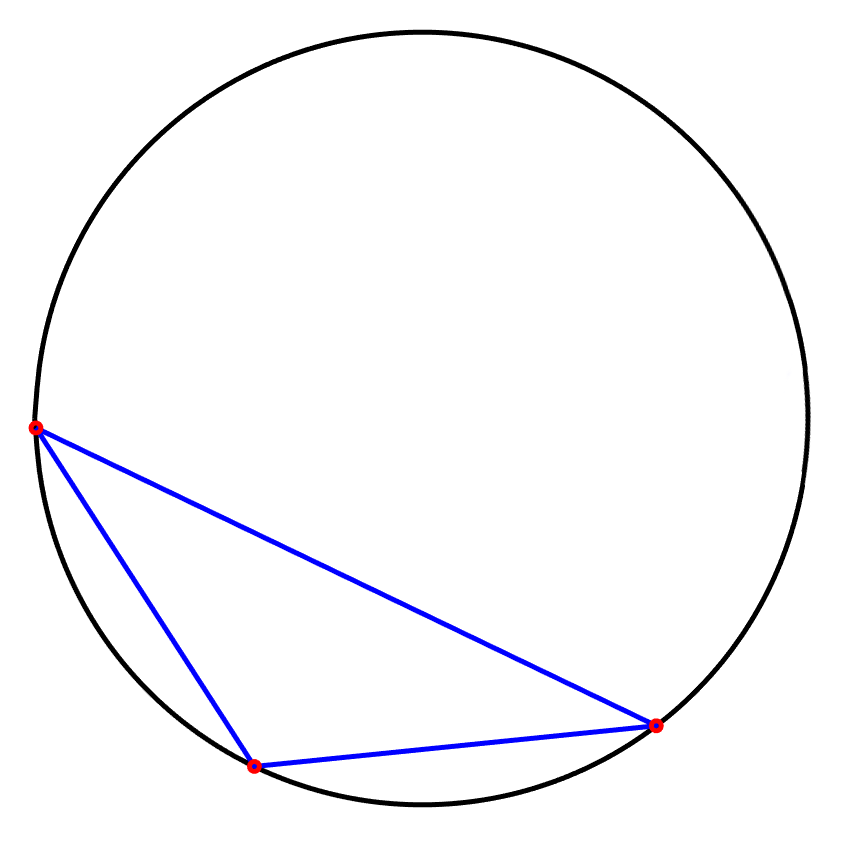
\includegraphics[width=0.4\textwidth]{./images/wpms/triang-insc.png}
%    \caption{Representation of the triangle obtained from the rolling points detected from the wheel profiles}
%    \label{fig:triang-inscritto}
%  \end{figure}
Hence, we can define the diameter $D$ of the circle circumscribed to the triangle as follows:
  \begin{equation*}
    D = \frac{a\cdot b\cdot c}{2A}
  \end{equation*}
and replacing $A$ with Equation \ref{eq:area}, we can conclude that:
  \begin{equation}
    D = \frac{2\cdot a\cdot b\cdot c}{\sqrt{( a + b + c )( - a + b + c )( a - b + c )( a + b - c )}}
    \label{eq:diam:erone}
  \end{equation}
~\\

As we have done for the model proposed in Chapter \ref{ch::model}, we are interested in determining the error made while we are evaluating this property of the wheel, and if possible, to develop a model that allows to determine the better configuration during the design of the system. Thus, we used the same approach as before, and the equation for the propagation error is:
  \begin{equation}
    \sigma_D = \sqrt{
      \left( \frac{\partial D}{\partial a} \sigma_a \right)^2 + 
      \left( \frac{\partial D}{\partial b} \sigma_b \right)^2 + 
      \left( \frac{\partial D}{\partial c} \sigma_c \right)^2
    }
    \label{eq:diam-prop-1}
  \end{equation}
However, we had some problems to evaluate the errors $\sigma_a$, $\sigma_b$ and $\sigma_c$. Each point used as vertex for the triangle, was obtained from a different laser-camera pair. Accordingly with what we have done in Chapter \ref{ch::model}, each of these pairs could be set in a different way, depending by the requirements, hence the weight of the noise in the final spot detection, can be different pair by pair.

To solve this problem we thought to project all the points in a common reference system, like the one shown in Figure \ref{fig:common-rs}.
  \begin{figure}[t!]
    \centering
    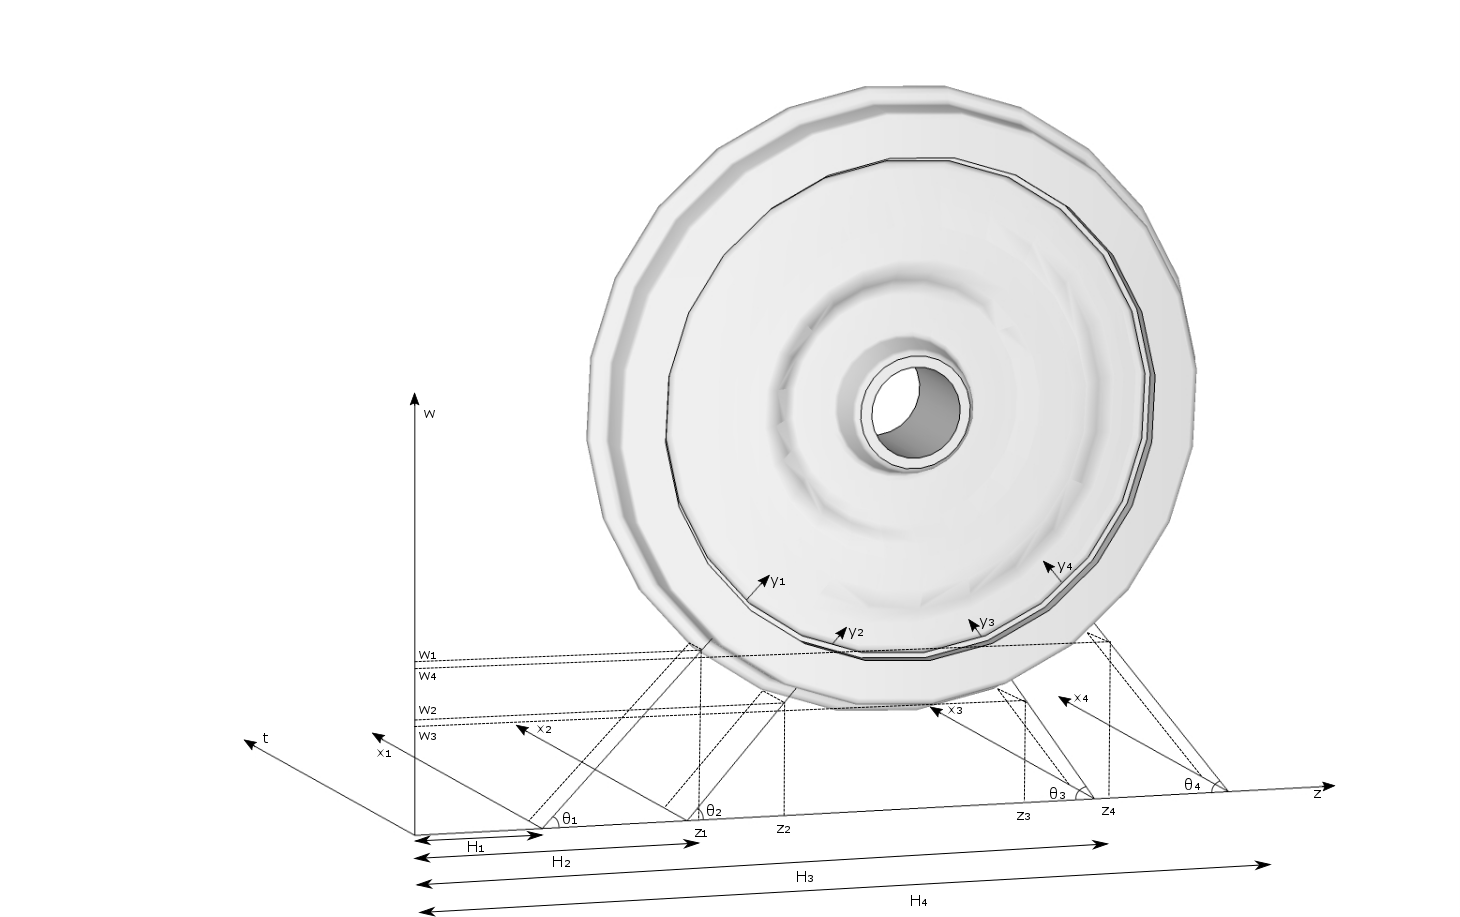
\includegraphics[width=\textwidth]{./images/wpms/diam_rs.png}
    \caption{Example of the common reference system used for all the detected rolling points}
    \label{fig:common-rs}
  \end{figure}
In this way, each vertex can be defined by a vector, starting from the laser projector to the point itself. We called this vector $y_i$. Using simple trigonometric relationships, we can decompose each vector in the its components $w_i$ and $z_i$ as follows:
  \begin{equation}
    \begin{matrix}
      w_i = y_i \cdot \sin \theta_i \\ \\
      z_i = y_i \cdot \cos \theta_i + H_i \\
    \end{matrix}
    \label{eq:components}
  \end{equation}
where $\theta_i$ is the triangulation angle and $H_i$ is the offset of the laser projector with respect to the origin of the coordinate system. At this point, it is simple to compute the edges length as:
  \begin{equation}
    \left\{
    \begin{matrix} 
      & a = \sqrt{(w_1 - w_2)^2 + (z_1 - z_2)^2} \\ \\
      & b = \sqrt{(w_2 - w_3)^2 + (z_2 - z_3)^2} \\ \\
      & c = \sqrt{(w_3 - w_1)^2 + (z_3 - z_1)^2}
    \end{matrix}
    \right.
    \label{eq:edges-len}
  \end{equation} \\
Hence, replacing in Equation \ref{eq:diam-prop-1} the results obtained in Equations \ref{eq:edges-len} and \ref{eq:components}, we can conclude that the error is propagated accordingly with:
  \begin{equation}
    \sigma_D = \sqrt{
      \sum_{i = 1}^3 \left( \frac{\partial D}{\partial y_i} \sigma_{y_i} \right)^2 + 
      \sum_{i = 1}^3 \left( \frac{\partial D}{\partial H_i} \sigma_{H_i} \right)^2 + 
      \sum_{i = 1}^3 \left( \frac{\partial D}{\partial \theta_i} \sigma_{\theta_i} \right)^2
    }
    \label{eq:diam-prop-2}
  \end{equation} \\
 
The last step, is linking the Equation \ref{eq:diam-prop-2} with the output of the Equations \ref{eq:radial-compensations}. In real conditions, the transformations between the laser-camera pairs and the common coordinate reference system are allowed by a second calibration process. As discussed in Section \ref{sec:teo-calibration}, the camera calibration can determine the intrinsic and extrinsic parameters of a single camera. However, this process can be modified in order to align two or more cameras at the same reference system, as in this case. \\
Ideally, the two reference systems are related to each other through a rototranslation, i.e. a linear transformation. This means that the vector $y_i$ remains the same, except for the values of its coordinates. Thus, we can determine the norm of $y_i$ as:
  \begin{equation*}
    |y_i| = \sqrt{x_w^2 + y_w^2 + z_w^2}
  \end{equation*}
where $\left( x_w, y_w, z_w \right)$ are the coordinates evaluated with Equations \ref{eq:radial-compensations}, and $z_w = 0$ accordingly with the fact that the laser plane is arbitrarily put at $0$. Now, it is simple to determine $\sigma_{y_i}$ as:
  \begin{equation*}
    \sigma_{y_i} = \sqrt{
      \left( \frac{\partial y_i}{\partial x_w} \sigma_{x_w} \right)^2 + 
      \left( \frac{\partial y_i}{\partial y_w} \sigma_{y_w} \right)^2
    }
    % = \frac{x}{\sqrt{x_w^2 + y_w^2}}
  \end{equation*}
where $\sigma_{x_w}$ and $\sigma_{y_w}$ are the value computed with Equations \ref{eq:err-radial-comp-xw} and \ref{eq:err-radial-comp-yw}, respectively. \\

Concerning the estimation of $\sigma_{H_i}$ and $\sigma_{\theta_i}$, the things are simpler. The errors of $H_i$ are a constructive parameters, i.e. we can set them reasonably, with respect to the requirements of product construction. Vice-versa, $\theta_i$ are the same triangulation angles used in Chapter \ref{ch::model}, thus $\sigma_{\theta_i}$ can be computed accordingly with Equation \ref{eq:det_a}.
